\subsection{Etape 3 : processus de sélection}
\vspace{1cm}

J’avais donc pour chaque match une liste d’arbitres habilités potentiels. La prochaine étape était donc de procéder aux désignations. \\

Contrairement aux matchs uniques, les matchs tournois doivent avoir un arbitre pour chaque groupe de trois matchs de la même poule. Il fallait donc prendre en compte différemment la sélection en fonction du type de match.

Autre contrainte mineure, il fallait que la désignation prenne en compte le nombre exacte d’arbitres pour chaque match.

\subsubsection{Matchs uniques}
\vspace{1cm}

La seule chose à prendre en compte pour la sélection des arbitres pour les matchs uniques était le nombre d’arbitres nécessaires pour chaque match. Cette donnée n’est pas explicite et dépend de la poule et du niveau du match. 
J’ai donc créé une méthode dans la classe \colored{DesignationsBase} qui permet de déterminer si un match demande deux arbitres ou non.

\begin{figure}[!h]
    \centering
    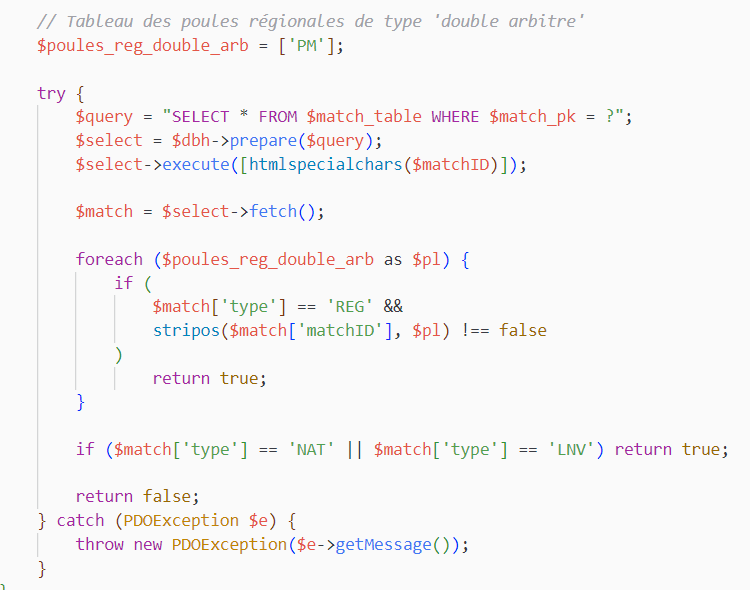
\includegraphics[width=0.75\linewidth]{double}
    \caption{Détermination du nombre d'arbitres pour le match}
\end{figure}

Le nombre d’arbitres est déterminé en fonction du niveau du match (régional ou national), et prend en compte les exceptions. \\

Une fois le nombre d’arbitres défini, la distance entre chaque arbitre potentiel est récupérée dans la base de données et associée avec les arbitres dans un tableau trié par distance croissante. Ce tableau final permet de procéder aux désignations de façon semi aléatoire en augmentant progressivement la probabilité de sélection des arbitres en fonction de leur distance avec le gymnase.

\begin{commentaire}
Un score aléatoire est attribué à chaque arbitre. Ce nombre aléatoire est compris entre 0 et 100, puis multiplié par une valeur allant de 2 à 0,5. Les arbitres voient leur score ajusté à la baisse entre ces deux valeurs en fonction de leur distance avec le gymnase.
Ceci induit alors que le score de l’arbitre le plus proche est multiplié par deux et celui du plus éloigné est divisé par deux.
\end{commentaire}

De cette façon, les arbitres dont la distance avec le gymnase est faible ont plus de chance d’être sélectionnés par l’algorithme, sans pour autant enlever complètement la probabilité de sélection des arbitres dont la distance est plus élevée.

Une fois un arbitre sélectionné, celui-ci est ensuite retiré du tableau global des arbitres disponibles du jour pour ne plus être resélectionné pour d’autres matchs le même jour.

\subsubsection{Matchs tournois}
\vspace{1cm}

Le processus de sélection des matchs tournois se rapproche de celui des matchs uniques.
La sélection reste semi aléatoire de façon à mettre l’accent sur les arbitres dont la distance avec le gymnase est plus faible.  \\

Cependant, par souci d’optimisation, il fallait pouvoir désigner un seul arbitre par paquet de trois matchs de la même poule d’un tournois. 
De cette façon, un arbitre se déplacerait pour arbitrer trois match consécutifs d’un tournois.

J’ai pris en compte cette différence en ajoutant quelques ligne de code permettant de désigner le même arbitre pour trois match consécutif de la même poule.